% !TeX spellcheck = en_US
% Chapter 1

%\chapter{Chapter Title Here} % Main chapter title
%
%\label{Chapter1} % For referencing the chapter elsewhere, use \ref{Chapter1} 

%----------------------------------------------------------------------------------------

% Define some commands to keep the formatting separated from the content 
\newcommand{\keyword}[1]{\textit{#1}}
\newcommand{\sm}[0]{$M_\odot$}
\newcommand{\todo}[1]{\texttt{\color{red}\#TODO: #1}}
%\newcommand{\file}[1]{\texttt{\bfseries#1}}
%\newcommand{\option}[1]{\texttt{\itshape#1}}

%----------------------------------------------------------------------------------------

\section{Galatic setup}
	\subsection{Units}
		Computer simulations are sensitive to rounding errors due to the lack of infinite precision when representing decimal numbers. Really small numbers as well as really big ones tend to have bigger errors than those close to the unity. \todo{include IEEE 754}
		
		Under the International System of Units, distances are measured on meters, times on seconds, and mass on kilograms, nevertheless black holes are too heavy to be measured on kilograms, galaxies sizes too big to be quantified on meters, and time scales too large for a second. Because of that, the following units will be used throughout this document:
		\begin{table}[h]
			\centering
			\caption{Natural units}
			\label{tb: units}
			\begin{tabular}{c|c}
				\hline
				\textbf{Physical property} & \textbf{unit} \\
				\hline
				Length & 1 kilo-parsec (kpc) \\
				Mass & $10^5$ solar masses ($10^5$ \sm) \\
				Time & 1 giga-year (Gyr) \\
				\hline
			\end{tabular}
		\end{table}		
		
		\subsubsection{Universal gravitational constant}
			First quantified by Henry Cavendish the gravitational constant has a value of $G_0 = 6.67408\times10^{-11}$ on SI units of m$^3$s$^{-2}$kg$^{-1}$. With the units of length, mass and time on \autoref{tb: units} the constant of gravity to be used is given by:
			\begin{equation}
				\small
				G = G_0 \left(\dfrac{1 \text{ kpc}^3}{\left(3.0857\times10^{19}\right)^3  \text{ m}^3}\right)\left(\dfrac{\left(3.154\times10^{16}\right)^2 \text{ s}^2}{1 \text{ Gyr}^2}\right)\left(\dfrac{1.98847\times10^{35} \text{ kg}}{10^5 M_\theta}\right) = 0.4493 \dfrac{\text{kpc$^3$}}{\text{Gy$r^210^5$\sm}}
			\end{equation}
			
		\subsubsection{Hubble constant}
	\subsection{Mass distributions}
		\begin{figure}[h]
			\centering
			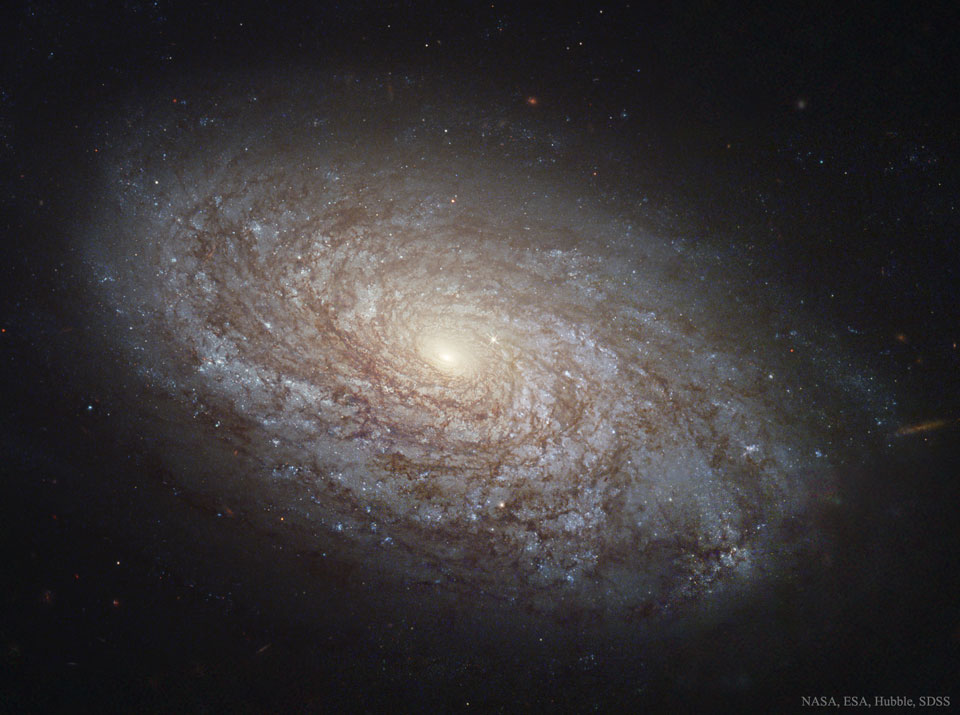
\includegraphics[width=0.7\linewidth]{Figures/NGC4414_modified}
		\end{figure}
	\subsection{Dark matter halo}
		For a dark matter halo following a NFW profile, the density at some distance $r$ is given by the formula:
		\begin{equation}
			\rho_\text{DM}(r) = \dfrac{\rho_0^\text{DM}}{\frac{r}{R_s}\left(1 + \frac{r}{R_s}\right)^2}
		\end{equation}
		
		Where $R_s$ and $\rho_0^\text{DM}$ are constants for a given dark matter halo.
		
		The cumulative mass within some radius $r$ is:
		\begin{equation}
			M_{DM} = \int\limits_0^{r} 4\pi {r'}^2\rho_\text{DM}(r')dr' = 4\pi\rho_0R_s^3\left[\ln\left(\dfrac{R_s + r}{R_s}\right) - \dfrac{r}{R_s + r}\right]
		\end{equation}
		
		Since the mass of dark matter of a single galaxy diverges for $r \rightarrow \infty$ there is a radius called $R_\text{vir}$, at which the density of the NFW profile is 200 times the critical density $\rho_\text{crit}$ the minimum density for an expanding universe.
		\begin{equation}
			R_\text{vir} = 200 \rho_\text{crit} = 200 \left(\dfrac{3H^2}{8\pi G}\right)
		\end{equation}
		
		Considering a concentration parameter $c(M_h, z)$ of dark matter in the halo, given by:
		\begin{equation}
			c(M_h, z) = c_0(z)\left(\dfrac{M_h}{10^{13}M_\theta}\right)^{\alpha(z)} \qquad \text{where $z$ is the redshift}
		\end{equation}
		
		where $\alpha(z)$ and $c_0(z)$ were fitted using simulation data to the following functions:
		\begin{equation}
			c_0(z) = \dfrac{4.58}{2}\left[\left(\dfrac{1 + z}{2.24}\right)^{0.107} + \left(\dfrac{1 + z}{2.24}\right)^{-1.29}\right]
		\end{equation}
		
		\begin{equation}
			\alpha(z) = -0.0965 \exp\left(-\dfrac{z}{4.06}\right)
		\end{equation}
		
		The concentration parameter of dark matter relates the viral radius $R_\text{vir}$ and the scale radius $R_s$ as:
		\begin{equation}
		R_\text{vir} = c(M_h, z)R_s
		\end{equation}

	
\section{Metodología}
%	El paso inicial consiste en generar un cuerpo con $10^8$ \sm usando la librer\'ia REBOUND, el cual tendr\'a la siguiente ecuaci\'on de movimiento:
	\begin{equation}
		\ddot{\vec{x}} = \left(-\dfrac{GM_h(x)}{x^2} + a_{DF}-\ddot{x}\dfrac{\dot{M_\bullet}}{M_\bullet} -qH^2x\right)\hat{x}
	\end{equation}
	
%	donde $M_h$ corresponde con la masa del halo de la galaxia, $a_{DF}$ con la aceleraci\'on debida a la fricci\'on din\'amica, la cual se modela usando la f\'ormula de Chandrasekhar para la materia oscura y el modelo h\'ibrido descrito por Choksi para la materia visible \cite{choksi2017recoiling}. El tercer t\'ermino tiene en cuenta la acreci\'on de masa por el agujero negro, y el \'ultimo la aceleraci\'on cosmol\'ogica.
%	
%	Dicha ecuaci\'on ser\'a integrada usando un esquema \textit{Leapfrog}, el cual se encuentra implementado en la librer\'ia REBOUND. Usando como condiciones iniciales $\vec{x} = (0,0,0)$ km y $\dot{\vec{x}} = (70, 0, 0)$ km$s^{-1}$, e intervalos de integraci\'on temporales de 1000 años, se busca reproducir los comportamientos observados por Choksi y colaboradores, para comprobar que el algoritmo implementado funcione de manera adecuada.
%	
%	Posteriormente ser\'an introducidas las modificaciones al potencial cambiando $M_h(x)$ por $M_h(x, y, z)$, donde los pesos de cada dimensi\'on ser\'an determinados de manera aleatoria para cada simulaci\'on. Al mismo tiempo se asignar\'an velocidades iniciales aleatorias, logar\'itmicamente espaciadas en el rango de 0 kms$^{-1}$ hasta 3000 kms$^{-1}$, sin ninguna direcci\'on preferente. Para cada sistema generado se realizar\'a la evoluci\'on en el tiempo usando integradores num\'ericos distintos. El tiempo aproximado de cada simulaci\'on se encuentra en el orden de 100$^6$ a\~nos, por lo cual ser\'an necesarias cerca de cien mil interaciones por cada conjunto de par\'ametros escogidos.
%	
%	Las simulaciones ser\'an realizadas en el cluster de la universidad (HPC) con el fin de paralelizar procesos, minimizando el tiempo de simulación y de esta forma lograr la mayor cantidad de simulaciones posibles, con el fin de obtener una cantidad significativa de datos de validación. A partir de estos, se obtendr\'an las distribuciones de probabilidad de los tiempos de retorno, y la cuantificaci\'on de la caoticidad de la trayectoria.